\documentclass{exam}

\usepackage{units} 
\usepackage{graphicx}
\usepackage[fleqn]{amsmath}
\usepackage{cancel}
\usepackage{float}
\usepackage{mdwlist}
\usepackage{booktabs}
\usepackage{cancel}
\usepackage{polynom}
\usepackage{caption}
\usepackage{fullpage}
\usepackage{xfrac}
\usepackage{enumerate}

\newcommand{\degree}{\ensuremath{^\circ}} 
\everymath{\displaystyle}

\printanswers

% \begin{figure}[H]
%   \centering
%   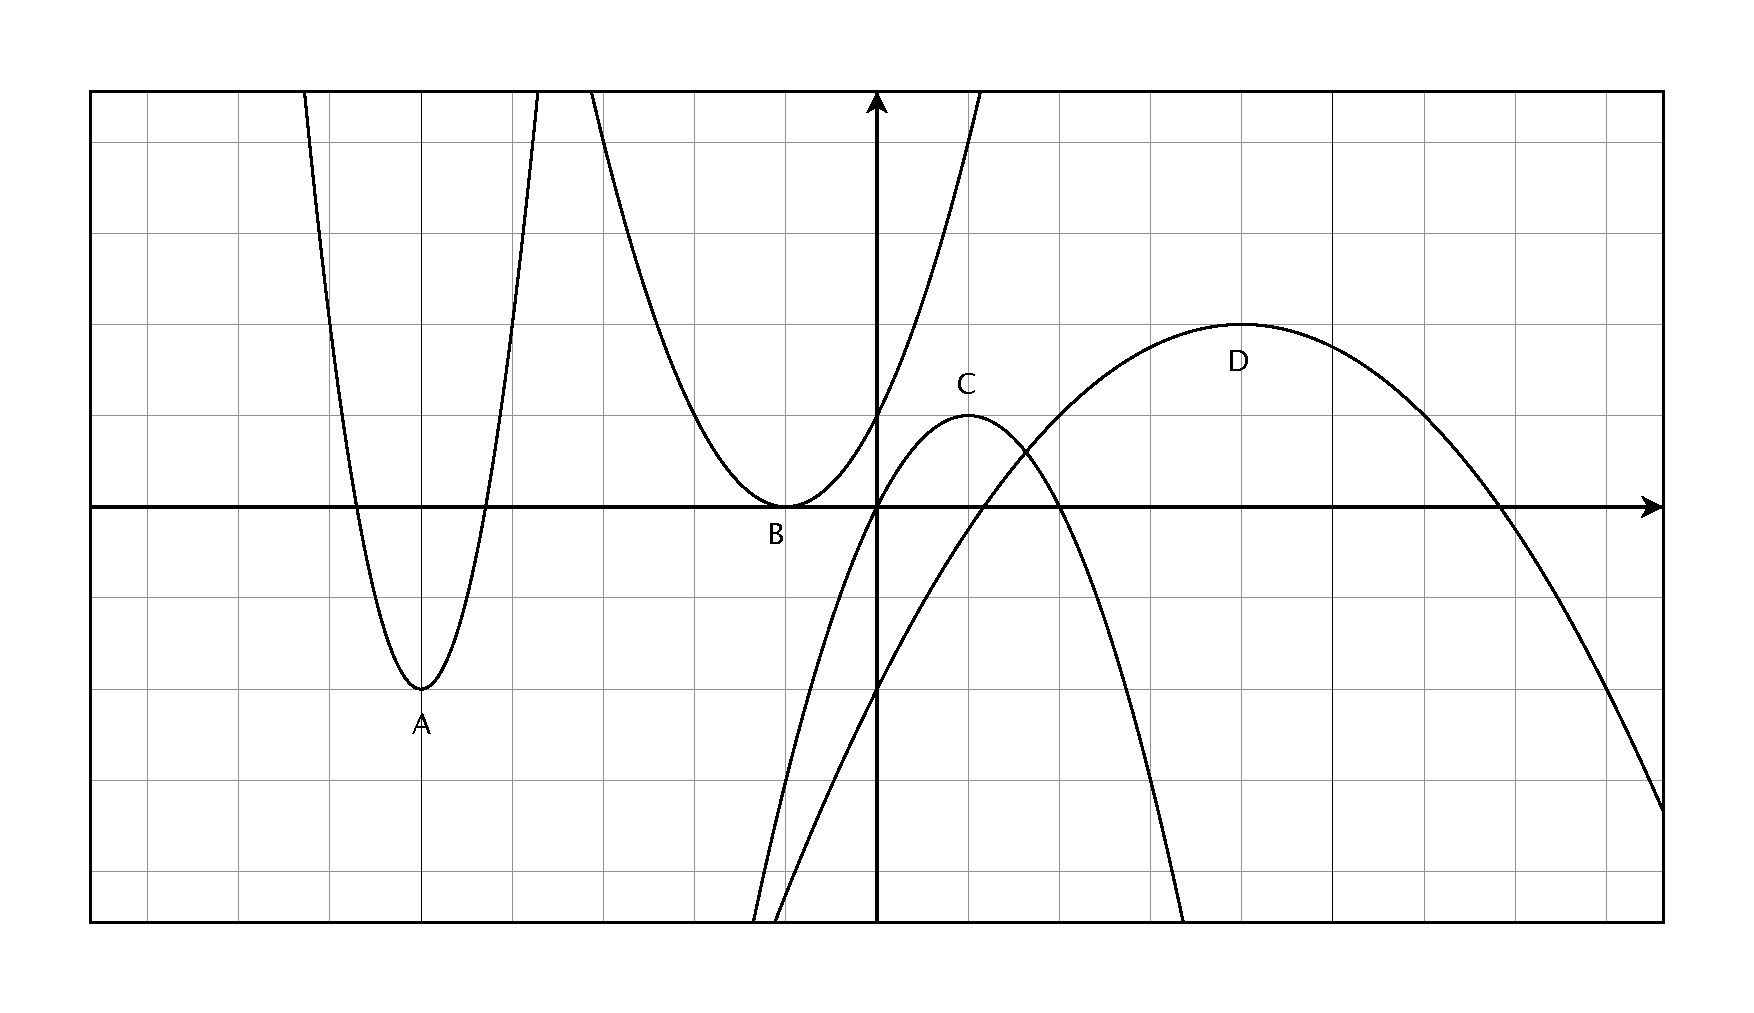
\includegraphics[scale=.3]{problem_7.eps}
%   \caption*{Problem 7}
% \end{figure}

% \begin{tabular}{cc}
% \toprule
% period & amplitude \\
% \midrule
%   $\pi$ & $2$ \\
% \bottomrule
% \end{tabular}

\title{Math 142 Notes \\ Section 5.3}

\date{\today}

\begin{document}

  \maketitle
  \tableofcontents

  \section{Periodicity}
  \begin{itemize}
    \item sine, cosine, etc., repeat as you go around the unit circle again
    \item $\sin(t \pm 2n \pi = \sin t$ for any integer $n$, etc.
    \item a function is periodic if there is some $p$ where $f(t + p) = f(t)$ for any value of $t$.  The smallest
      $p$ that works is the {\em period} of $f$.
    \item to graph a periodic function, you only need one period
    \item The period of sine, cosine, secant, and cosecant is $2 \pi$.  The period of tangent and cotangent is
      $\pi$
  \end{itemize}

  \section{Graphing Sine and Cosine} 

  \subsection{Basic Graph}
  \begin{itemize}
    \item draw single period of sine using known points
    \item draw single period of cosine using known points
    \item shift up and down by adding a constant
  \end{itemize}

  \subsection{Amplitude}
  For vertical scaling: $f(x) = a \sin x$, $|a|$ is the {\em amplitude } which determines how big the peaks and valleys
  are.

  \subsection{Period}
  For horizontal scaling, $f(x) = \sin kx$, period is $\frac{2 \pi}{k}$.  The graph repeats every 
  $\frac{2 \pi}{k}$

  The graph shrinks if $k > 1$ and stretches if $k < 1$ (small period means high frequency).

  \subsection{Phase}
  To shift left/right, add/subtract a constant: $f(x) = \sin(x - b)$.  $b$ is the {\em phase}.

  \subsection{General Form}
  \[
    y = a \sin k(x - b)
  \]

  \begin{itemize*}
    \item $|a|$ is the amplitude
    \item $\frac{2 \pi}{k}$ is the period
    \item $b$ is the phase shift

    \item to graph one period, graph from $b$ to $b + \frac{2 \pi}{k}$
  \end{itemize*}



\end{document}
